% \newcommand{\prototitle}{Versuch 2 - Statistik}
% \newcommand{\Fachbereich}{Praktikum Messtechnik}
% \input{../packages/tu_header}

\newcommand{\institut}{Institut f\"ur Telekommunikationssysteme}
\newcommand{\fachgebiet}{Nachrichten\"ubertragung}
\newcommand{\veranstaltung}{Praktikum Nachrichten\"ubertragung}
\newcommand{\pdfautor}{\"Ozg\"u Dogan (326 048), Boris Henckell (325 779)}
\newcommand{\autor}{\"Ozg\"u Dogan (326 048)\\ Boris Henckell (325 779)}
\newcommand{\gruppe}{Gruppe: }
%\newcommand{\betreuer}{Betreuer: Mahmoud Felk}


\newcommand{\pdftitle}{Nachrichten\"ubertragung\ Praktikum\ 02}
\newcommand{\prototitle}{Praktikum 02 \\ Zufallsexperiment und Rauschkanal}


\input{../../packages/tu_header_8}


% \lstlistoflistings
\definecolor{darkgray}{rgb}{0.95,0.95,0.95}
\definecolor{darkolivegreen}{HTML}{01a801}
\definecolor{functionsBlue}{HTML}{32b9b9}
\definecolor{variableRed}{rgb}{1,0,0}
\definecolor{stringBrown}{HTML}{bc8e8e} % f geht nicht

\lstset{
        %\lstset{extendedchars=true} % Umlaute an der richtigen stelle und nicht am Anfang ausgeben
        %basicstyle=\footnotesize\ttfamily,
        basicstyle=\small,
        %
        inputencoding=utf8,
        %
        tabsize=4,
        showspaces=false,
        showtabs=false,
        showstringspaces=true, % no special string spaces
        %
        backgroundcolor=\color{darkgray}, % background
        stringstyle=\color{stringBrown}\fseries, % Strings
        keywordstyle=\color{functionsBlue}\bfseries, % keywords Blau
        identifierstyle=\color{variableRed}, % variablen
        commentstyle=\color{darkolivegreen}, %  comments
        %
        breaklines=true,
        %
        numbers=left,
        numberstyle=\tiny,
        stepnumber=1,
        numbersep=7pt,
        %
        frame=single,
        columns=flexible,
        %
        xleftmargin=-2cm,
        xrightmargin=-1.5cm,
        %
        language=Matlab
}

%---------------------------------------------------------------------
%---------------------------------------------------------------------
%---------------------------------------------------------------------
\section{Einleitung}

    In diesem Praktikumstermin haben wir uns mit den Themen Verteilungsdichtefunktionen und rauschbehafteter
    Übertragungskanal beschäftigt. Dazu haben wir zuerst mit Hilfe von Matlab verschiedener Zufallsexperimente
    simuliert, danach deren Verteilungsdichtefunktionen bestimmt und miteinander verglichen.
    Anschließend haben wir mit dem Telecommunications Trainer einen rauschbehafteten Übertragungskanal ausgemessen und
    die Dämpfungseigenschaften sowie die Rauschcharakteristik bestimmt.


\section{Vorbereitungsaufgaben}

    \begin{quote}
    Die Vorbereitungsaufgabe lautet, die Varianz von gleichverteiltem weißen Rauschen $N$ mit der
    Verteilungsdichtefunktion $p_{N(n)} = \frac{1}{2A} \sqcap_{2A} (n)$ zu berechnen.\\
    Zuerst berechnen wir den Mittelwert $\mu$:
   	\begin{equation*}
    	\begin{split}
    		\mu &= \int_{-\infty}^{+\infty} n \frac{1}{2A} \sqcap_{2A} (n) \mathrm dn\\
    		&= \int_{-A}^{+A} n \frac{1}{2A} \mathrm dn\\
    		&= \left[ \frac{1}{2A} \frac{1}{2} n^2 \right]_{-A}^{+A}\\
    		&= \frac{1}{4A} (A^2-(-A)^2)\\
    		&= 0
    	\end{split}
    \end{equation*}
    
    Dannach berechnen wir die Leistung des Signals$P$:\\
    \begin{equation*}
    	\begin{split}
    		P &= \int_{-\infty}^{+\infty} n^2 \frac{1}{2A} \sqcap_{2A} (n) \mathrm dn\\
    		&= \int_{-A}^{+A} n^2 \frac{1}{2A} \mathrm dn\\
    		&= \left[ \frac{1}{2A} \frac{1}{3} n^3 \right]_{-A}^{+A}\\
    		&= \frac{1}{6A} (A^3-(-A)^3)\\
            &= \frac{2A^3}{6A} = \frac{1}{3} A^2\\
    	\end{split}
    \end{equation*}
    
    Mit diesen Werten läßt sich die Varianz wie folgt berechnen:
    \begin{equation*}
    	\begin{split}
    		\sigma^2 &= P - \mu^2\\
    		&= \frac{1}{3} A^2 - 0 = \frac{1}{3} A^2
    	\end{split}
    \end{equation*}
	\end{quote}
         	


%--------------------------------------------------------------------
%-------------------------------------------------------------------- 
\section{Verteilungsdichtefunktion}
\begin{quote}
	
	\subsection{Theorie}
    \begin{quote}
        Bei einer Verteilungsdichtefunktion handelt es sich um eine Funktion mit deren hilfe man die Wahrscheinlichkeit
        eines Ereignissintervalls bestimmen kann. Hierfür wird die Verteilungsdichtefunktion über dieses
        Ereignissintervall integriert. Diese Art der Darstellung von Wahrscheinlichkeitsereignissen bietet sich
        besonders bei stetigen Verteilungen an.\vspace{1em}
        
        In dem Fall einer stetigen Verteilung ist die Wahrscheinlichkeit für das Auftreten eines ganz speziellen
        Ereignisses immer gleich null. Die Wahrscheinlichkeit für das Auftreten eines Erignissintervalls, das dieses
        spezielle Ereigniss enthält, ist jedoch größer null.\\
        Ein Beispiel hierfür ist die Verspätung von Zügen. Die Wahrscheinlichkeit, dass ein Zug exakt $5$ min Verspätung
        hat ist gleich null, da dieses Ereigniss nicht eintrifft sobald die Züge in Ihrer Verspätung auch nur um $1$
        nanosekunde abweichen. Jedoch lässt sich die Wahrscheinlichkeit bestimmen, das ein Zug eine Verspätung zwischen
        $4,55$ min und $5,05$ min hat.\vspace{1em}
        
    \end{quote}
	
	\subsection{Simulation meherer Zufallsexperimente in Matlab}
    \begin{quote}
        Um mehrere Verteilungsdichtefunktionen zu plotten haben wir meherere Zufallsereignisse mit Matlab simuliert.\\
        Zu Beginn des Praktikums wurde uns hierfür die Datei Aufgabe1.m zur verfügung gestellt, die wir im Verlauf
        stückweise erweitert haben.\\
        In der Ursprungsversion simuliert Aufgabe1.m ein Zufallsereigniss mit 10000 Würfen eines Würfels und plottet
        anschließend das Histogramm dieser Simulation.\\
        \subsubsection{10000 facher  Wurf eines Würfels}
        \begin{quote}
            Für die erste Teilaufgabe haben wir die Datei Aufgabe1.m so ergänzt, dass die Anzahl der Treffer durch die
            Anzahl der Würfe geteilt wird. Dadurch errechnen wir uns die Häufigkeitsverteilung normiert wird und so ihre
            Summe genau 1 ist. Das Ergebniss haben wir plotten lassen.

        \end{quote}
        
        \subsubsection{10000 facher Wurf zweier Würfel}
        \begin{quote}
            In der zweiten Teilaufgabe haben wir die Simulation soweit verändert, dass bei jedem Wurf zwei Würfel
            simmuliert wurden deren Augenzahl aufsummiert wurden. Damit auch der zweite Würfel unabhängig simuliert wird haben wir einen zweiten Vektor
            erstellt mit einem zufälligen $10000$-fachen Würfelereigniss und die beiden Vektoren addiert. In hinblick auf die
            folgende Aufgabe, bei der wesentlich mehr Würfel pro wurf addiert werden sollten, wurde uns aber auch beigebracht,
            dass die rand-funktion schon eine Lösung für dieses Problem integriert hat. Und desshalb haben wir anstatt des
            zweiten Vektors einfach den zweiten Parameter der rand-funktion auf zwei gestellt und somit unabhängige Würfel
            simuliert.\\
            Auch von dieser Simulation haben wir die normierte Häufigkeitsdichte errechnet und
            plotten lassen.\\
        \end{quote}
        
        \subsubsection{10000 facher Wurf meherer Würfel}
        \begin{quote}
            Um den zentralen Grenzwertsatz der Statistik nachzuvollziehen erhöhen wir in der dritten Teilaufgabe
            schrittweise die Anzahl der Würfel, die miteinander addiert werden. Anschließend erstellen wir jeweils die
            Häufigkeitsdichte sowie die dazupassende geschätzte Verteilungsdichtefunktion.
            Laut Grenzwertsatz erwarten wir, dass sich die resultierende Verteilungsdichtefunktion sich an eine Gaußverteilung anpasst.
        \end{quote}        
    \end{quote}
	
	\subsection{Auswertung}
    \begin{quote}
        Da es sich bei dieser Simulation um ein Diskretes ereigniss handelt werden die daraus resultierenden
        Häufigkeitsverteilungen selbstverständlich auch diskret sein. Eine Verteilungsdichtefunktion ist hingegen eine
        stetige Funktion. Daher lässen sich die beiden Funktionen nur an den Diskreten Punkten miteinander
        vergleichen.\\
        Ansonsten sit für alle Simulationen zu erwarten, dass sich die Häufigkeitsverteilungen den geschätzten
        Verteilungsdichtefunktionen grob ähneln werden.
        
        \subsubsection{10000 facher Wurf eines Würfels}
        \begin{quote}
                In dem Zufallsexperiment gehen wir davon aus, dass jede Zahl auf dem Würfel gleich wahrscheinlich
                gewürfelt werden kann. Außerdem wird das Experiment mit $10000$ Würfen häufig genug durchgeführt um zu
                einer aussagekräftigen Verteilung zu kommen. Daher erwarten wir eine gleichmäßig verteilte
                Häufigkeitsverteilung mit einem jeweiligen Wert von $\frac{1}{6}$ bzw. $0.16$.\\
                
                
                \begin{figure}[H] \centering
                    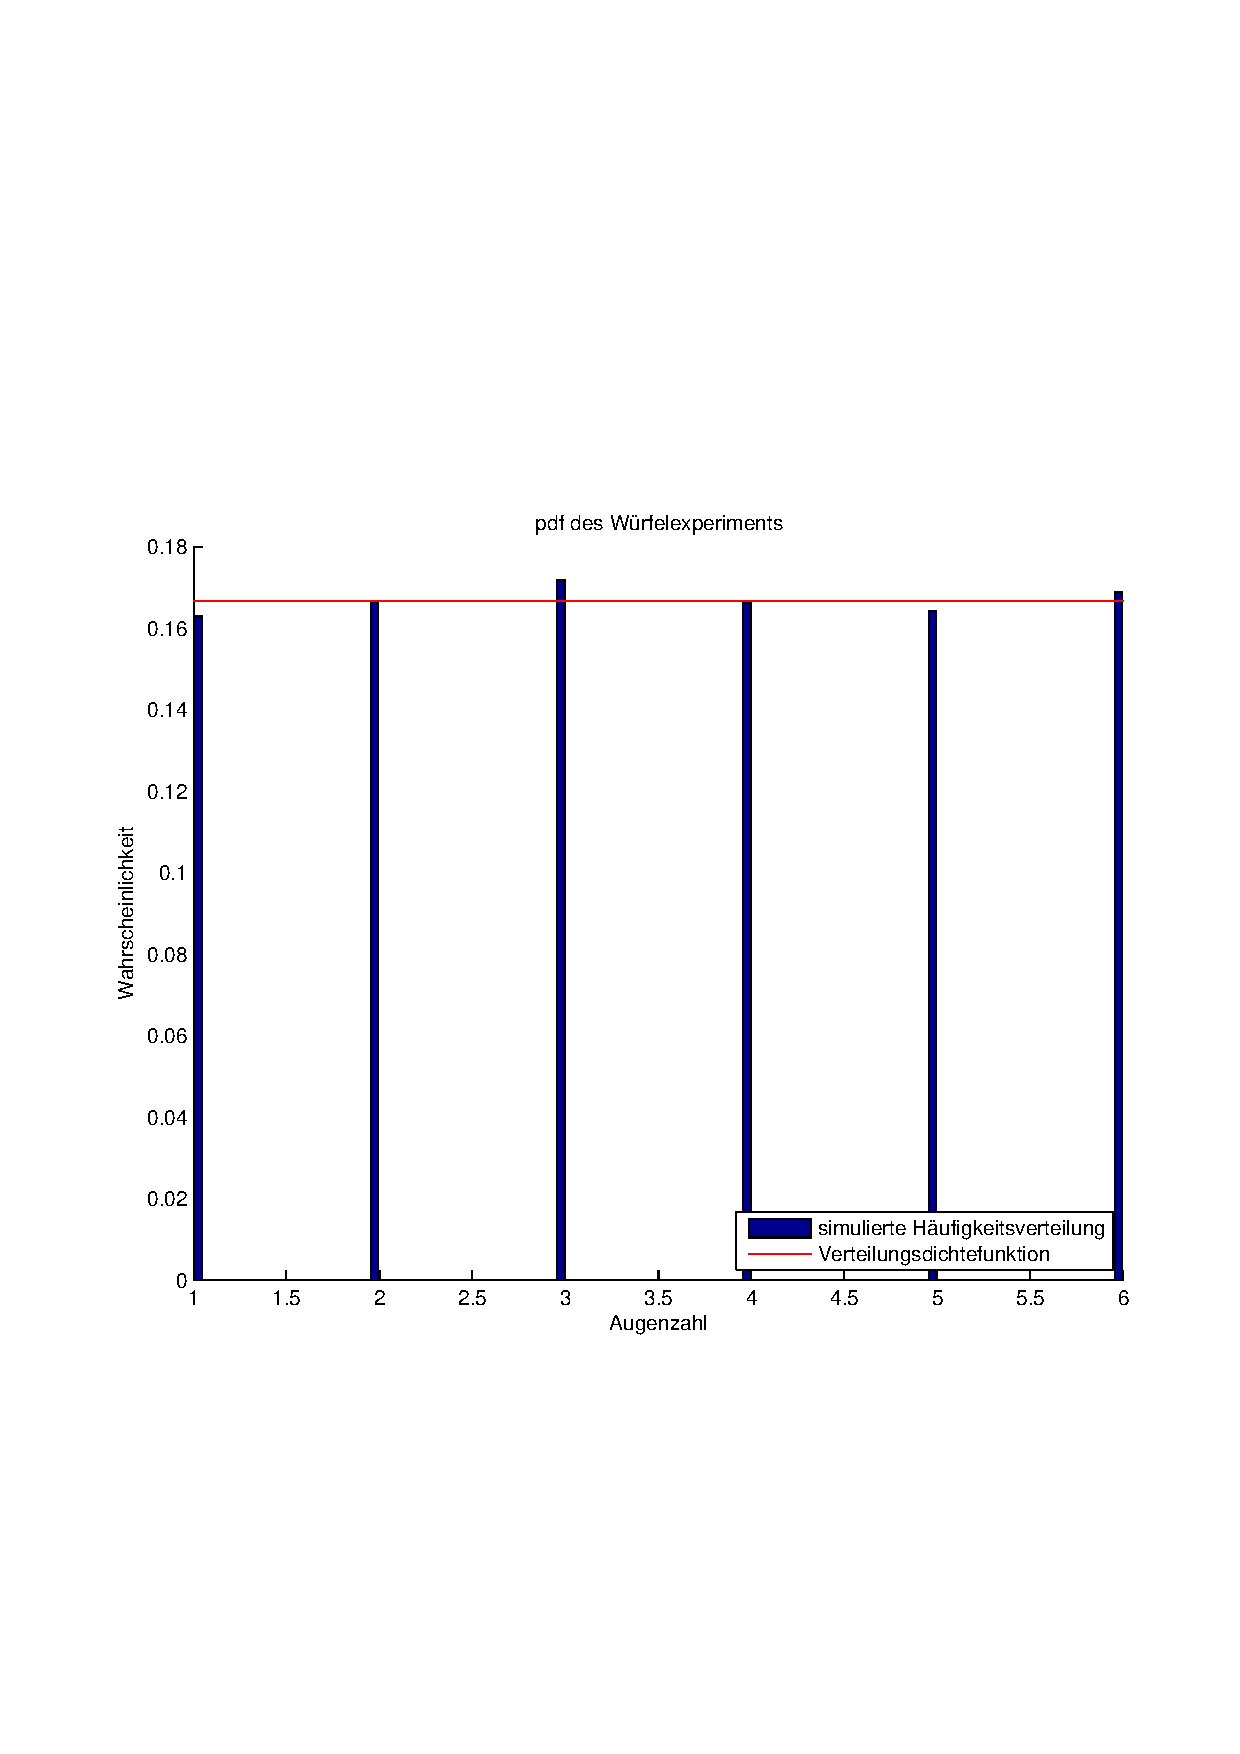
\includegraphics[scale=0.5, trim = 2cm 6.5cm 1.5cm 8.5cm, clip]{./Bilder/1wuerfelpdf}
                        \caption{Häufigkeitsverteilung 1 Würfel 10000 Würfel}
                \end{figure}
                
                Die Simulierte Häufigkeitsverteilung entspricht annähernd unseren Erwartungen. Auffällig ist jedoch,
                dass die Zahlen $3$ und $6$ ein wenig häufiger und die Zahlen $1$, und $6$ ein wenig seltener gewürfelt
                wurden als erwartet.
                Diese Abweichung erklären wir uns mit damit, dass es sich ein statistisch unabhängiges Experiment
                handelt. Daher können einige Zahlen häufiger gewürfelt werden als andere.\\
                Je mehr Würfe wir simulieren würden desto mehr müssten sich die Simulierten Werte an die erwarteten
                anpassen.\\
        \end{quote}
        
        \subsubsection{10000 facher Wurf zweier Würfel}
        \begin{quote}
            Die Verteilungsdichtefunktion von zwei bzw. mehreren unabhängigen Ereignissen lässt sich auch als Faltung
            der einzelnen Verteilungsdichtefunktionen darstellen. In Falle des einfachen Würfelwurfes hat sich die
            Verteilungsdichtefunktion als Rechteck herausgestellt. Die Faltung von zwei Rechtecken ergint wiederum ein
            Dreieck. Für die Verteilungsdichtefunktion von zwei Würfeln deren Augenzahlen addiert werden erwarten wir
            daher eine Dreieckförmige Verteilungsdichtefunktion.\\
            Die erwartete Dreieckförmige Verteilungsdichtefunktion lässt sich auch auf andere Weise erschließen. Die
            möglichen Ereignisse dieser Simulation sind die Zahlen von $2$ bis $12$. Wobei es für die beiden äußeren
            Ereignisse jeweils nur eine mögliche kombination der zwei Würfel gibt. Für das Ereigniss $7$ gibt es
            hingegen $6$ verschiedene Würfelkombinationen. Daher ist das Würfeln einer $7$ auch $6$ mal Wahrscheinlicher
            als das Würfeln einer $2$ oder $12$.\\
            
                \begin{figure}[H] \centering
                    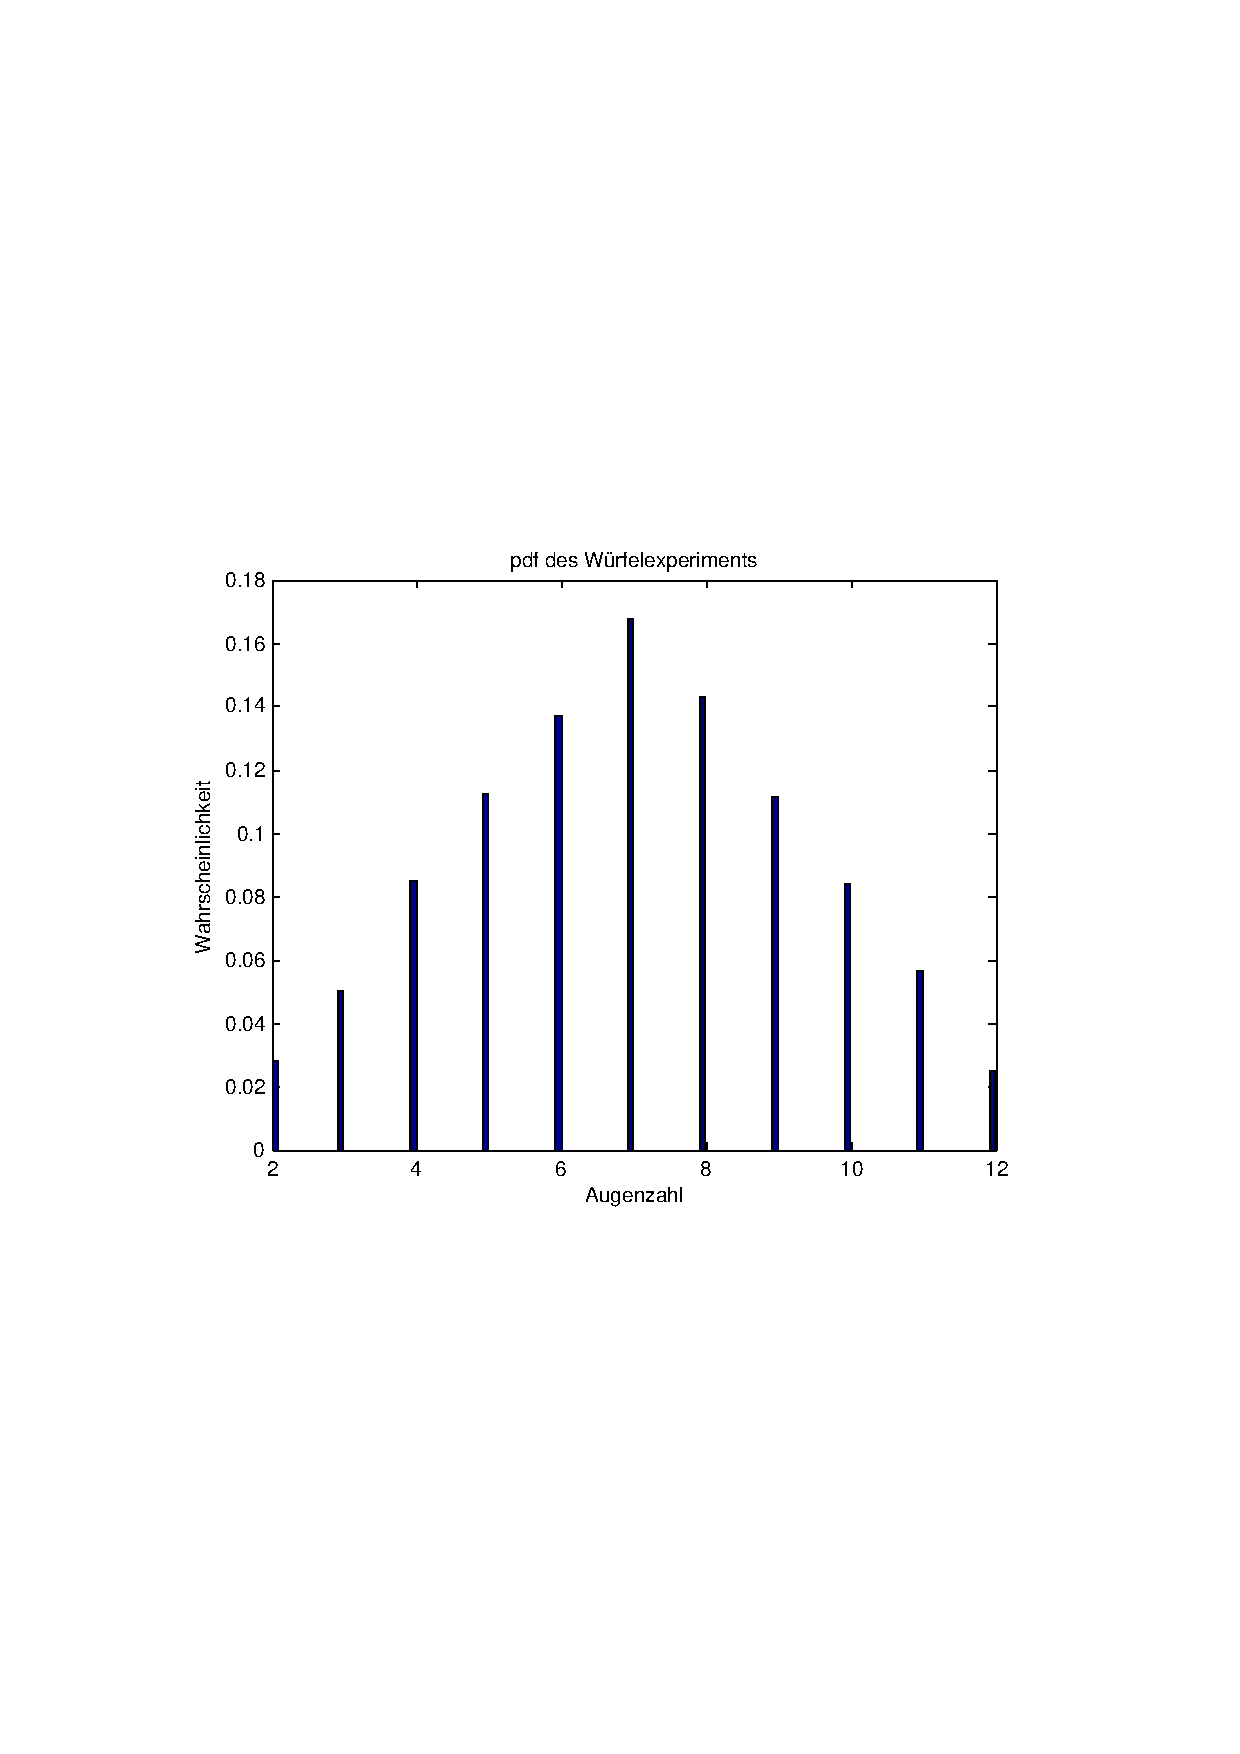
\includegraphics[scale=0.5, trim = 2cm 6.5cm 1.5cm 8.5cm, clip]{./Bilder/2wuerfelpdf}
                        \caption{Häufigkeitsverteilung 2 Würfel 10000 Würfel}
                \end{figure}
            
            Auch in dieser Simulation sind einige Abweichungen zu erkennen jedoch verhält sich die Simulation
            größtenteils wie erwartet.\\       
        \end{quote}
        
        \subsubsection{10000 facher Wurf mehrerer Würfel}
		\begin{quote}
			Genau wie die Verteilungsdichtefunktion von zwei unanbhängigen Ereignissen sich aus der Faltung der einzelnen
			Verteilungsdichtefunktionen ergibt, ergibt sich die Verteilungsdichtefunktion von mehreren unabhängigen Ereignissen
			von der Faltung ihrer einzelnen Verteilungsdichtefunktionen.\\
			Laut zentralem Grenzwertsatz erwarten wir, dass sich die Resultierenen Verteilungsdichtefunktionen immer mehr einer
			Normalverteilung annähern. Genauer gesagt erwarten wir eine annäherung an die Gaußnormalverteilung.

                        %4 Grafiken:
            \begin{center}
            \begin{tabular}{ll}

            \hspace{-14em}
                \begin{minipage}{0.6\textwidth}

                    \begin{figure}[H]
                        \label{fig:}
                        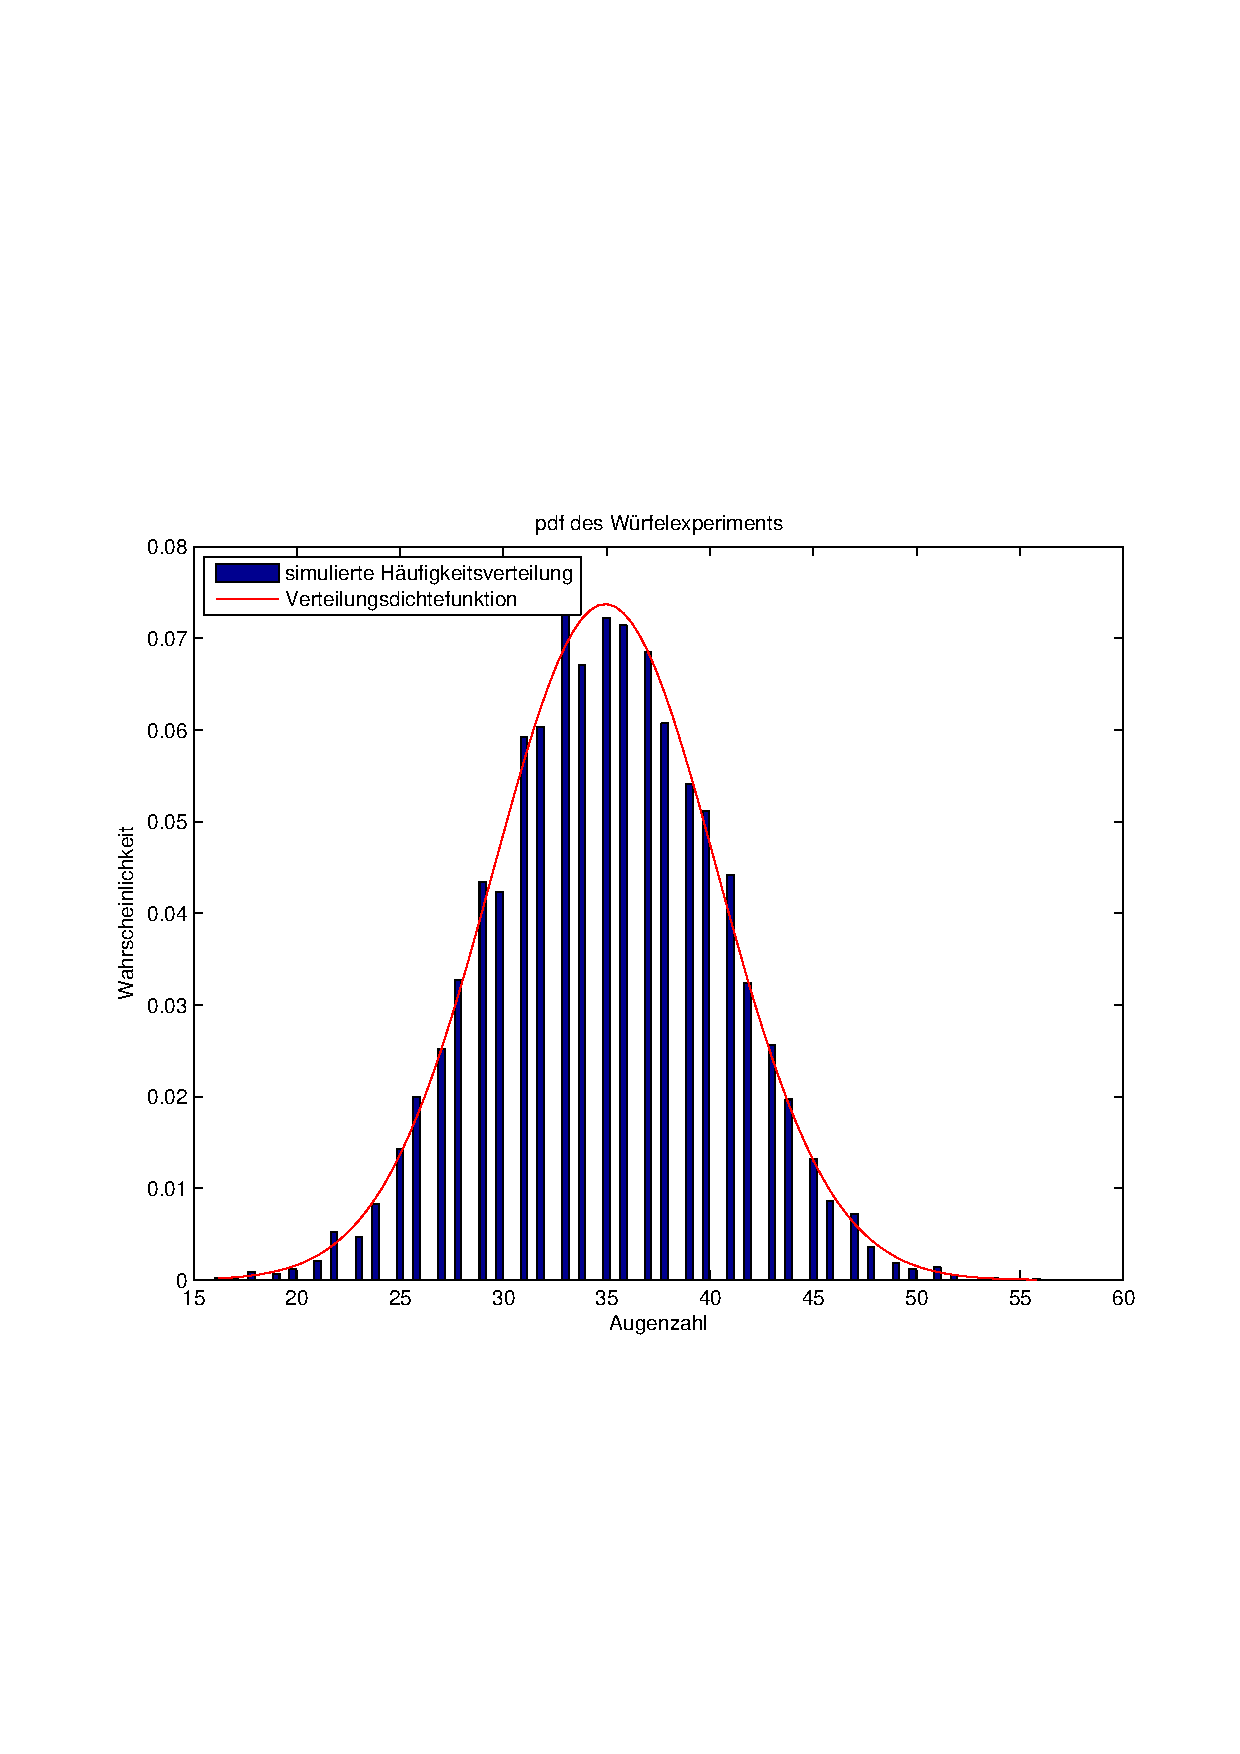
\includegraphics[scale=0.5, trim = 2cm 6.5cm 1.5cm 8.5cm, clip]{./Bilder/10wuerfelpdf} %FIXME
                        % [width=640px, height=474px]
                        \caption{PDF 10 Würfel 10000 Würfe}
                    \end{figure}

                \end{minipage}
                \begin{minipage}{0.6\textwidth}

                     \begin{figure}[H]
                        \label{fig:}
                        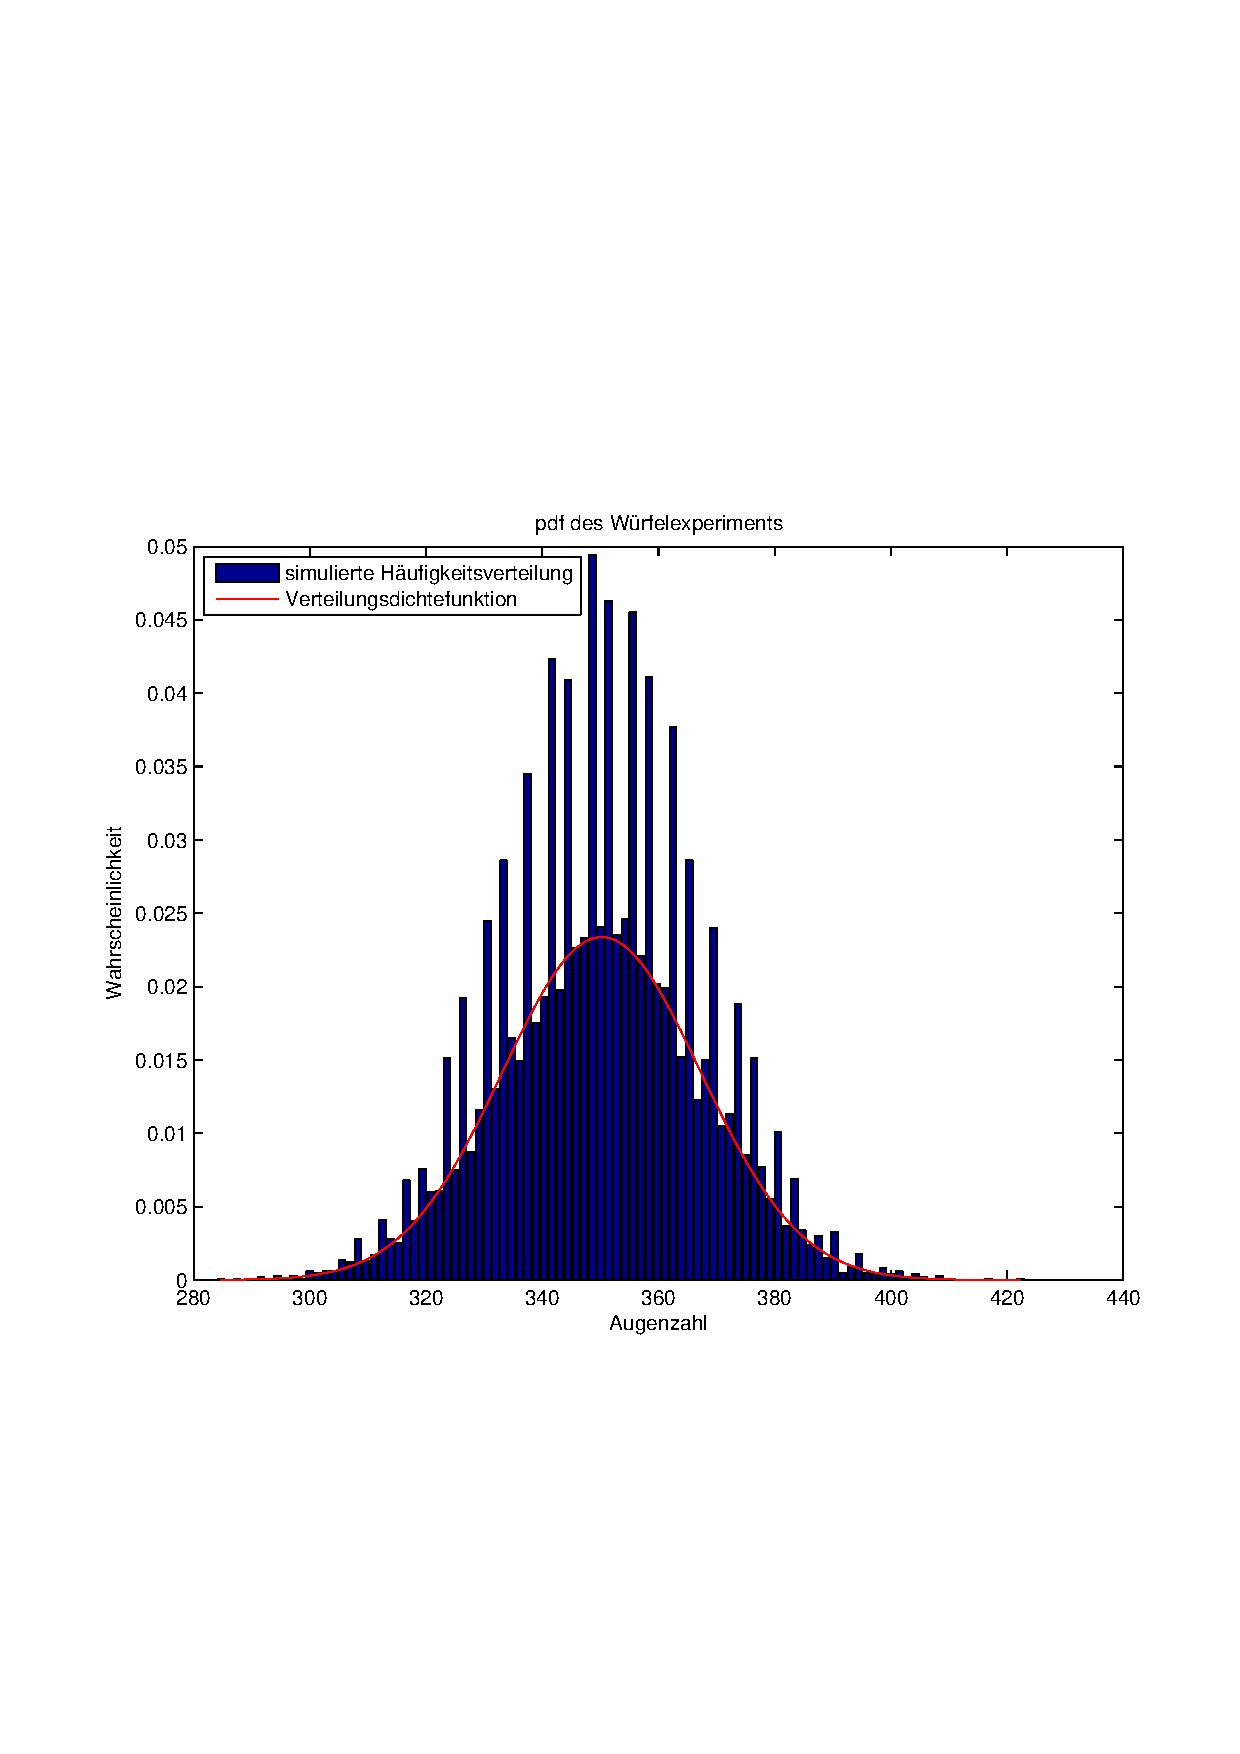
\includegraphics[scale=0.5, trim = 2cm 6.5cm 1.5cm 8.5cm, clip]{./Bilder/100wuerfelpdf} %FIXME
                        % [width=640px, height=474px]
                        \caption{PDF 100 Würfel 10000 Würfe}
                    \end{figure}
               \vspace{-1.5em}

                \end{minipage}

            \end{tabular}
            \end{center}

                        %4 Grafiken:
            \begin{center}
            \begin{tabular}{ll}

            \hspace{-28em}
                \begin{minipage}{0.6\textwidth}

                    \begin{figure}[H]
                        \label{fig:}
                        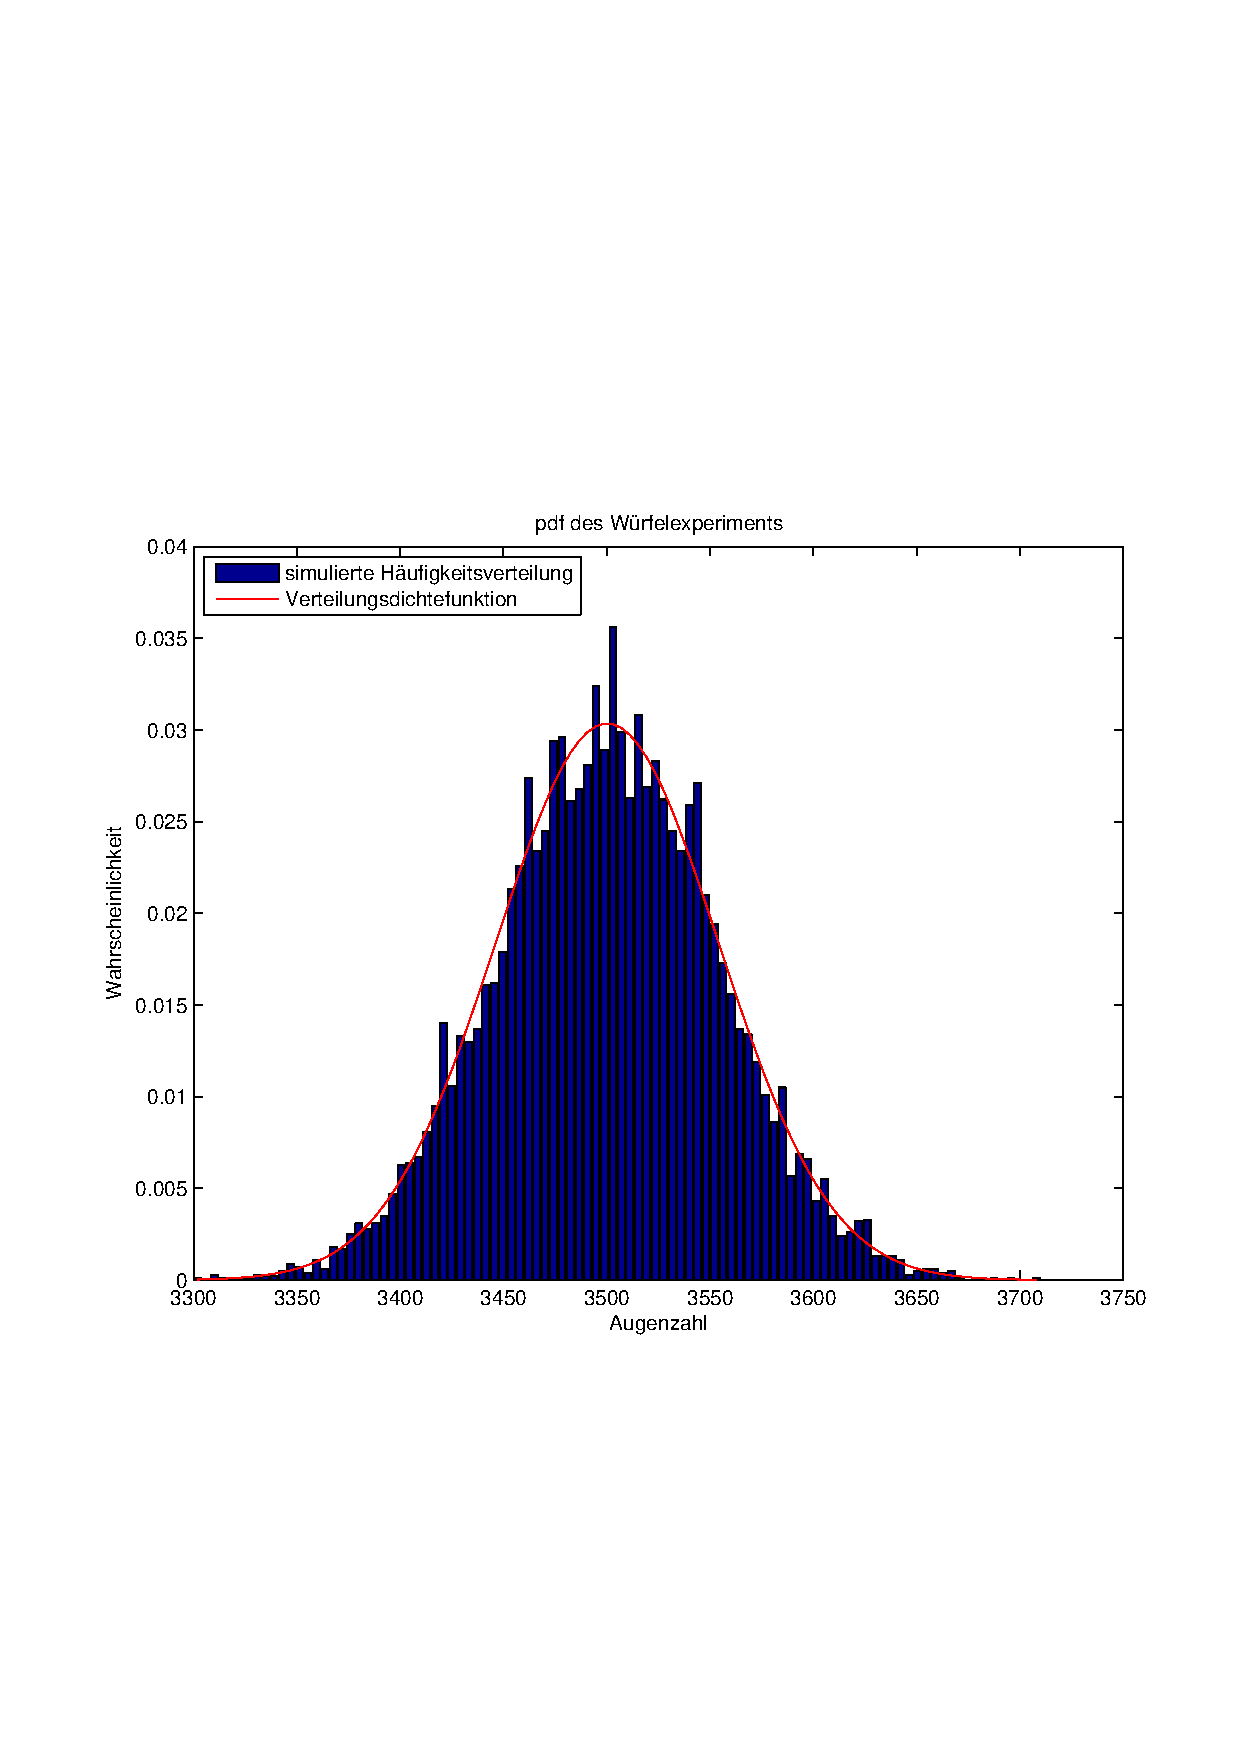
\includegraphics[scale=0.5, trim = 2cm 6.5cm 1.5cm 8.5cm, clip]{./Bilder/1000wuerfelpdf} %FIXME
                        % [width=640px, height=474px]
                        \caption{PDF 1000 Würfel 10000 Würfe}
                    \end{figure}

                \end{minipage}

            \end{tabular}
            \end{center}			
			
                Die Häufigkeitsverteilungen aus den drei Simulationen bestätigen die Vermutung, dass die Verteilungen
                sich immer mehr einer Gaußnormalverteilung anpassen.\\
                Besonders bei den $100$ Würfeln und den $1000$ Würfeln sind einige starke Abweichungen zu beobachten. Es
                ist auffällig, dass sie so stark ausfallen. Jedoch würden wir sie, wie auch die male davor, so erklären,
                dass es um ein statistisch unabhängiges Experiment handelt bei dem einige Zahlen häufiger gewürfelt
                werden als erwartet.
		\end{quote}
    \end{quote}
\end{quote}
%--------------------------------------------------------------------
%--------------------------------------------------------------------
\section{Rauschbehafteter Übertragungskanal}
\begin{quote}
	\subsection{Theorie}
    \begin{quote}
        Bei der Übertragung eines Signals über einen Rauschbehafteten Kanal wird dieses Signal durch Dämpfung und
        Rauschen beeinflusst. Rauschen wirkt sich negativ auf die Übertragung aus, da sich das Rauschen auf das
        Nutzsignal addiert und es so verändert. Je höher die Amplitude des Rauschens desto mehr stört das Rauschen
        das Nutzsignal.\\
        Eine Möglichkeit die Auswirkung von Rauschen auf ein Signal zu erfassen ist der
        Signal-Rausch-Abstand(SNR).
        Zur Errechnung des SNR wird die Leistung des Signals ins Verhältniss zu der Leistung des Rauschens gesetzt.
        
        \begin{equation*}
        	\begin{split}
        		SNR = \frac{P_{Signal}}{P_{Rauschen}}
        	\end{split}
        \end{equation*}
        
        Je größer die Amplitude des Rauschens wird desto kleiner wird der Signal-Rausch-Abstand, was negativ ist.\\
        Um den Signal-Rausch-Abstand bestimmen zu können benötigt man selbstverständlich gezielte Informationen über das
        Nutzsignal sowie das Rauschsignal. 
    \end{quote}
    
    \subsection{Durchführung}
    \begin{quote}
        Um einen Rauschbehafteten Übertragungskanal zu simulieren haben wir an dem Telecommunications Trainer ein
        Pseudozufälliges Signal erzeugt. Dieses Signal besitzt einen Mittelwert der $\neq$ null ist.\\
        Zu diesem Signal haben wir anschließend additiv Rauschen hinzugefügt. Beim ersten Durchgang $-20dB$, beim
        zweiten $-6dB$ und beim letzten $0dB$. Alle drei Rauschsignale sind Mittelwertfreie Signale. Sie stellen Weißes
        Rauschen dar mit einem Effektivwert von $0,5 V$ ($-20dB$), $2,45V$ ($-6dB$)  sowie $4,96 V$ ($0 dB$).
        Dannach haben wir das Originalsignal sowie das verrauschte Signal mit Hilfe des USB Oszilloskops aufgenommen. 
        Da das Eingangssignal einen Mittelwert $\neq$ null hat, das Rauschen jedoch ein Mittelwertfreies Signal
        darstellt, wissen wir, dass jede Abweichung des Mittelwertes zwischen dem Eingangssignal und dem Ausganssignal
        auf die Dämpfung des Kanals zurückzuführen ist. Daher vergleichen wir die Mittelwerte des Einganssignals und des
        Ausgangssignals miteinander. Der Korrekturfaktor $\alpha = \frac{mean(A)}{mean(B)}$, der an das Ausgangssignal
        ranmultipliziert wird, korrigiert somit die Dämpfung des Kanals.\vspace{1em}
        
        Nach dieser Korrektur haben wir die Häufichkeitsdichteverteilung des Rauschens bestimmt und geplottet.
        Abschließend haben wir noch das Signal-Rausch-Verhältniss der gemessenen Signale bestimmt. Dazu haben wir die Energie des
        Eingangs- und Ausgangssignal bestimmt und aus dem Verhältniss das Signal-Rausch-Verhältniss bestimmt.\\
        Für die Berechnung des SNR wird ursprünglich die Leistung der beiden Signale benötigt. Die Leistung
        Zeitdiskreter Signale werden folgendermaßen bestimmt:
        \begin{equation*}
            \begin{split}
                P_u(n_1, n_2) := \frac{1}{n_2 - n_1 + 1} \sum_{k=n_1}^{n_2} u^2 (k)
            \end{split}
        \end{equation*}
        
        Die Variablen $n_1,n_2$ beschreiben zusammen das Zeitintervall des Signals. Da das Eingangssignal und das
        Ausgangssignal unserer Messung über das selbe Zeitintervall bestimmt wird kürzen sich bei der Berechnung des SNR
        dieses Zeitintervall gegenseitig raus und es reicht mit dem Energieverhältniss zu rechnen.\\

        
    \end{quote}
    
    \subsection{Auswertung}
    \begin{quote}
        Von den Häufigkeitsverteilungen der drei Rauschsignalen erwarten wir mit zunehmendem Rauschen eine zunehmend
        breiter werdende Häufigkeitsverteilung. Außerdem erwarten wir zunehmend
        schlechtere Signal-Rausch-Verhältnisse, welches sich durch niedrigere SNR Werte zeigen sollte.\vspace{1em}
        
        Hier die Ergebnisse der Messung:
        
               \begin{center}
               \begin{tabular}{ll}
        
               \hspace{-4.5cm}
                   \begin{minipage}{0.6\textwidth}
        
                       \begin{figure}[H]
                           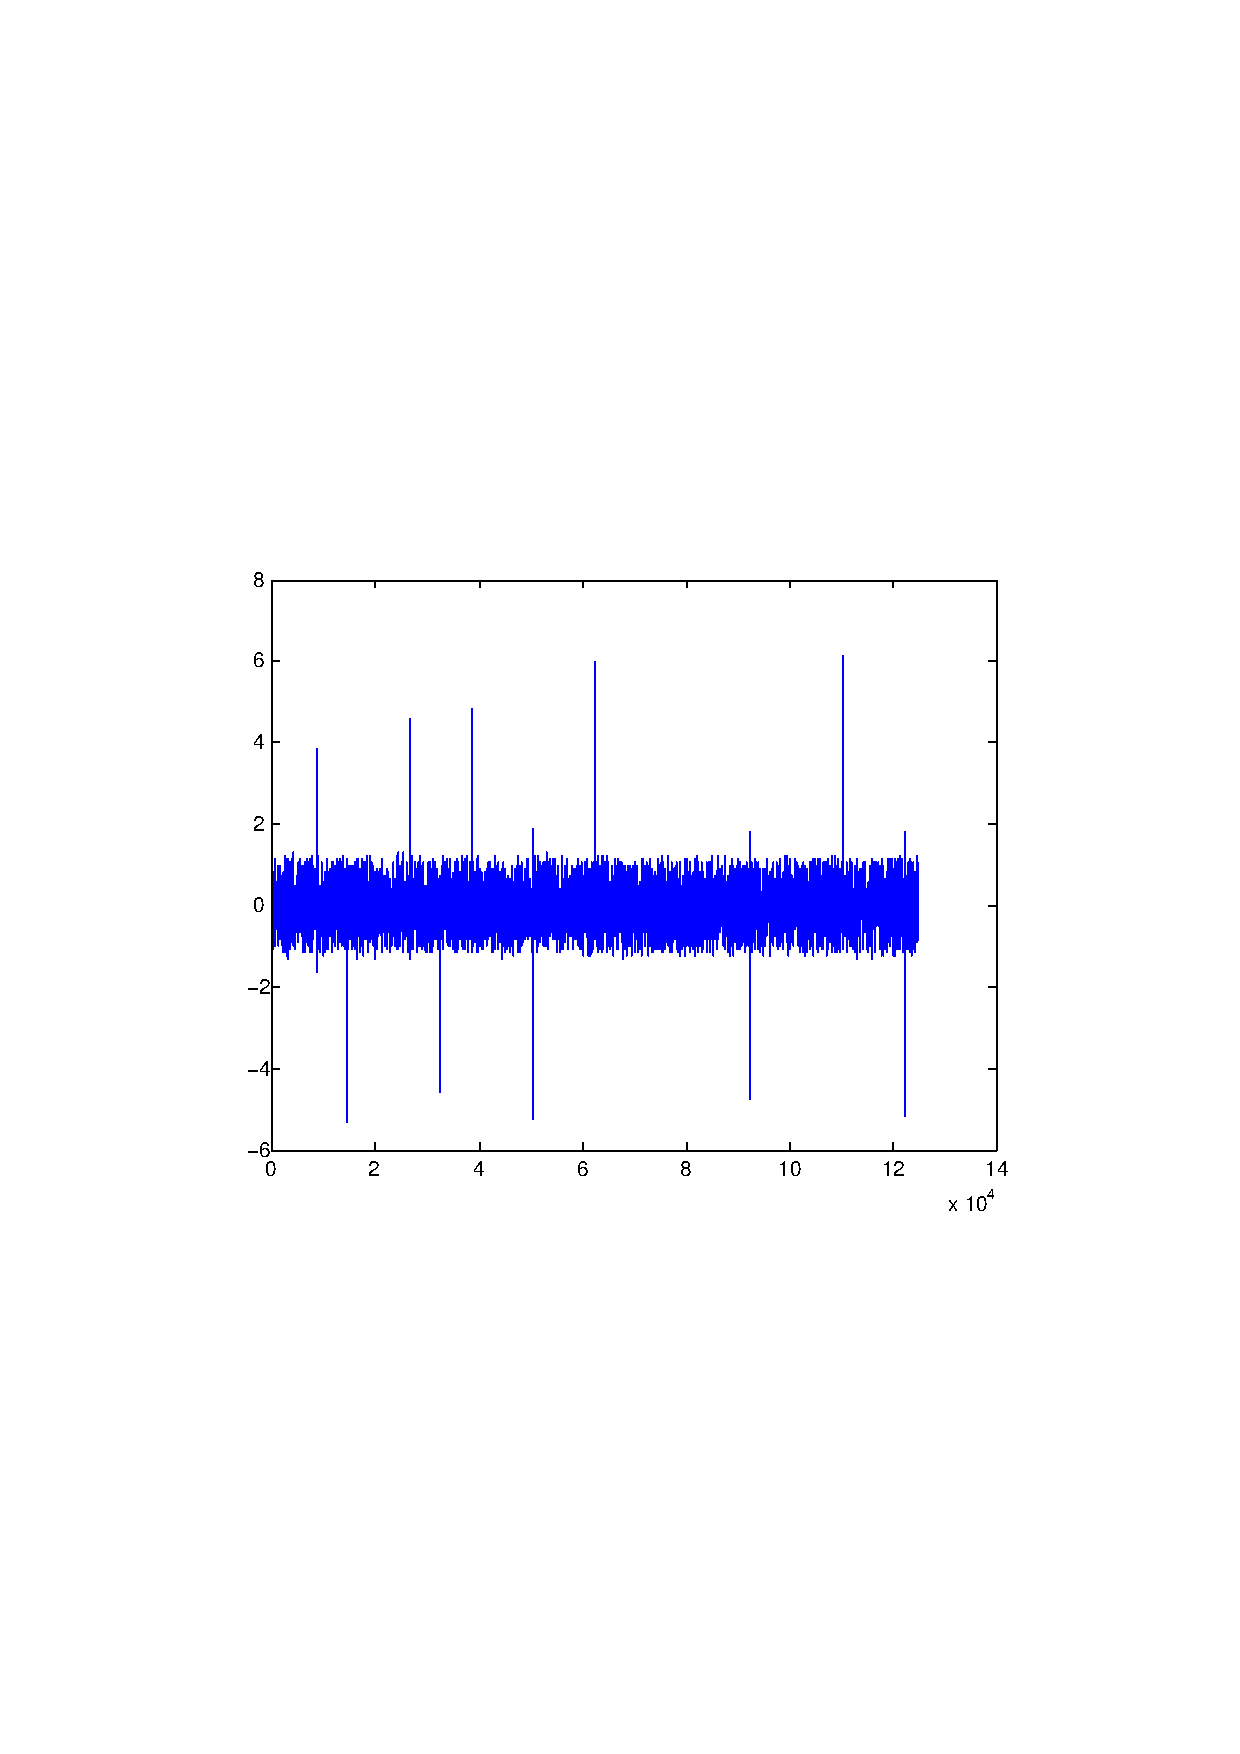
\includegraphics[scale=0.6, trim = 35mm 85mm 40mm 95mm, clip]{./Bilder/Rauschen-20dB}
                           \caption{-20dB Rauschen}
                       \end{figure}
        
                   \end{minipage}
        
                   \begin{minipage}{0.6\textwidth}
                       \begin{figure}[H] 
                           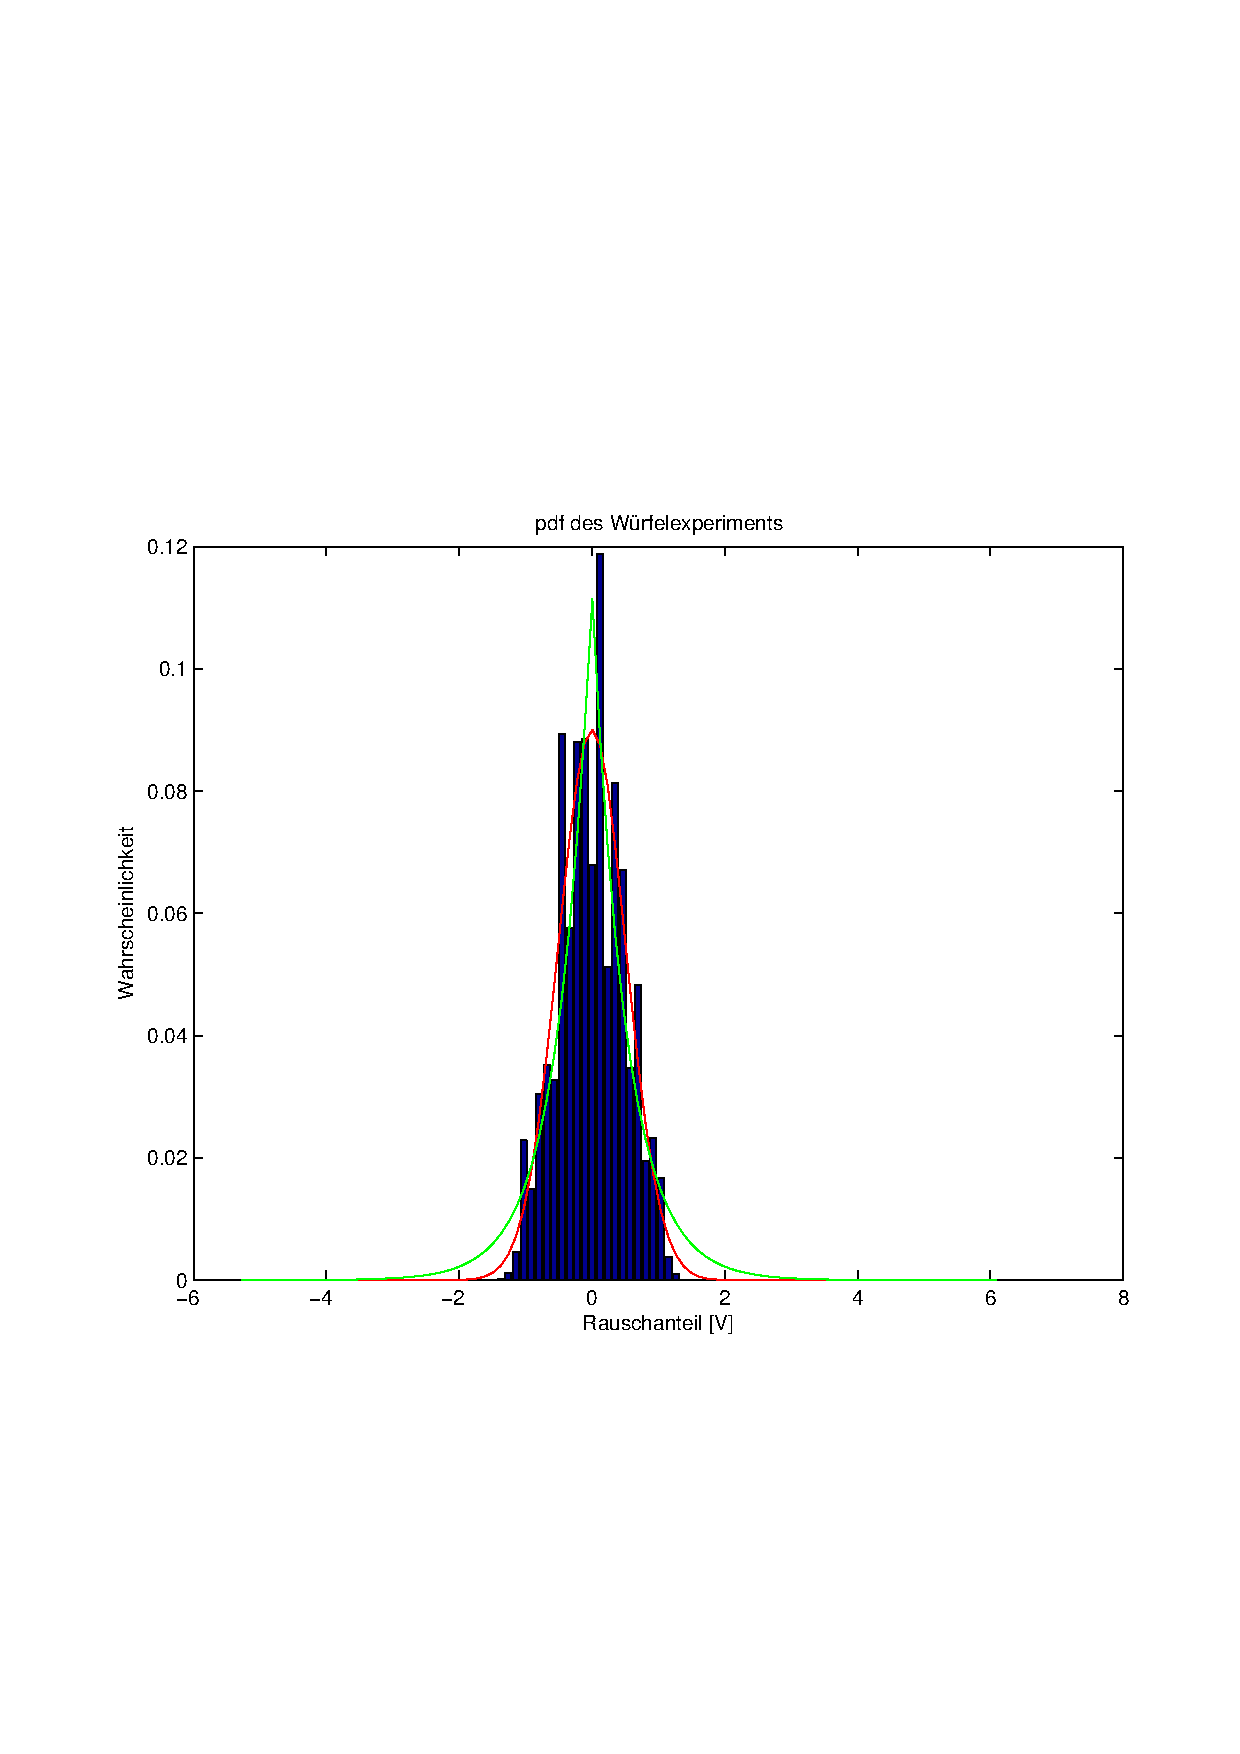
\includegraphics[scale=0.49, trim = 10mm 65mm 10mm 85mm, clip]{./Bilder/PDFRauschen-20dB}
                           \caption{Häufigkeitsverteilung -20dB Rauschen}
                       \end{figure}
        
                   \end{minipage}
        
               \end{tabular}
               \end{center}
        
                       \begin{center}
               \begin{tabular}{ll}
        
               \hspace{-4.5cm}
                   \begin{minipage}{0.6\textwidth}
        
                       \begin{figure}[H]
                           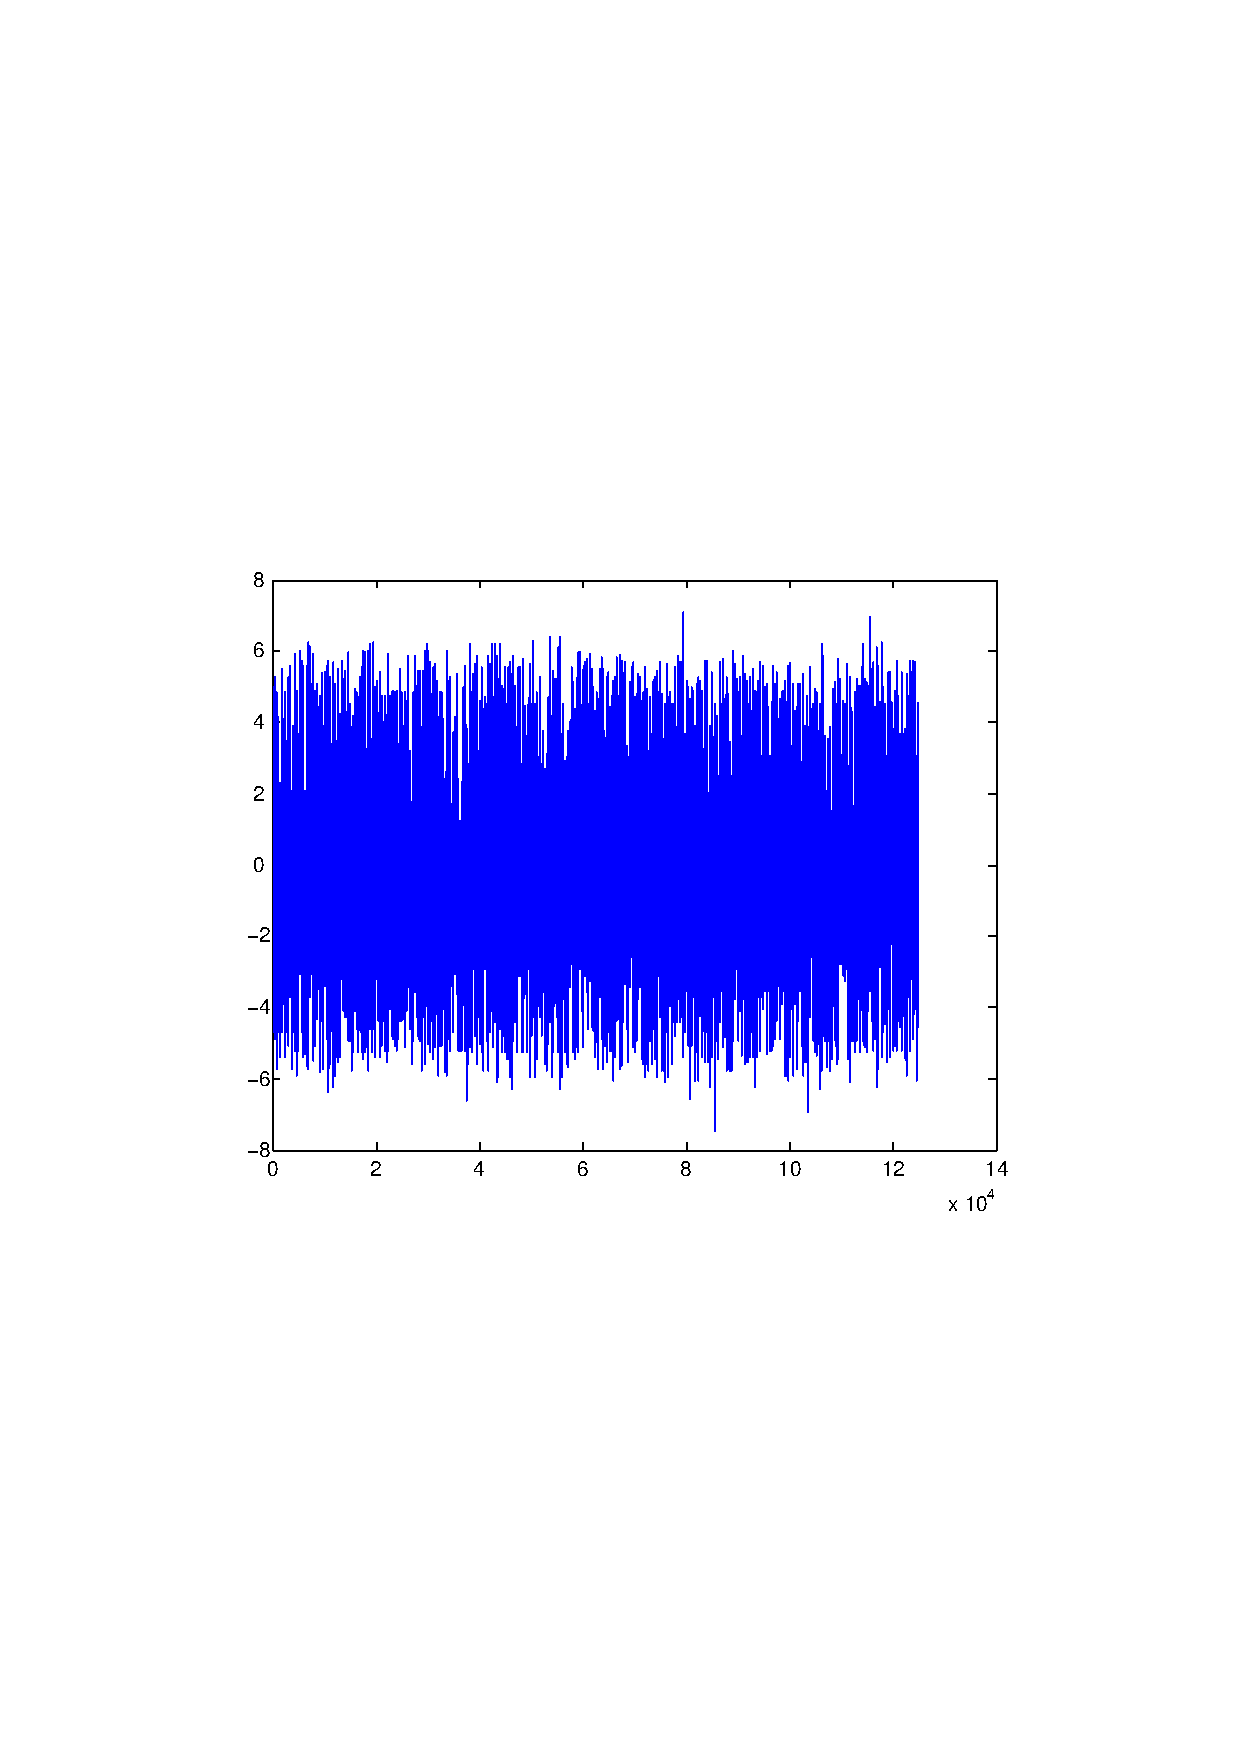
\includegraphics[scale=0.6, trim = 35mm 85mm 40mm 95mm, clip]{./Bilder/Rauschen-6dB}
                           \caption{-6dB Rauschen}
                       \end{figure}
        
                   \end{minipage}
        
                   \begin{minipage}{0.6\textwidth}
                       \begin{figure}[H]
                           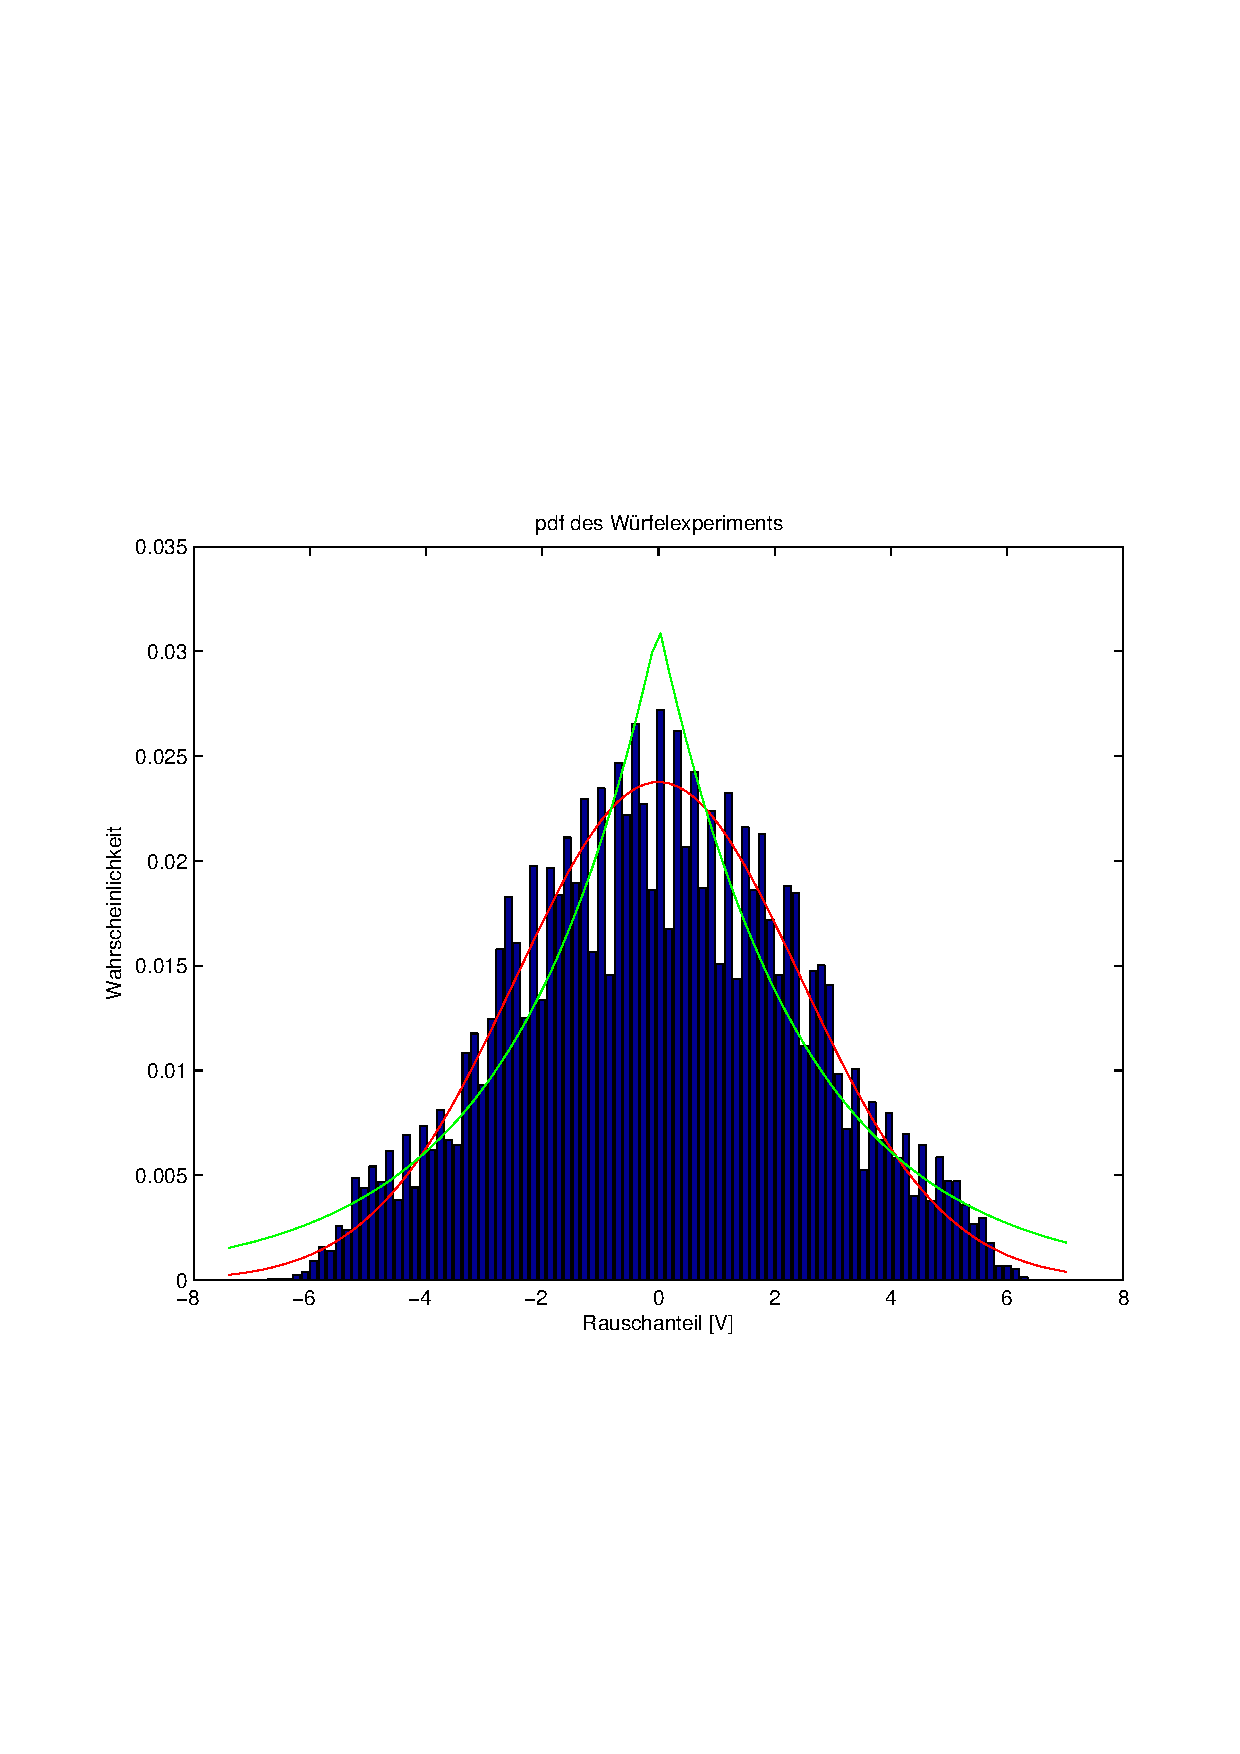
\includegraphics[scale=0.49, trim = 10mm 65mm 10mm 85mm, clip]{./Bilder/PDFRauschen-6dB}
                           \caption{Häufigkeitsverteilung -6dB Rauschen}
                       \end{figure}
        
                   \end{minipage}
        
               \end{tabular}
               \end{center}
        
                      \begin{center}
               \begin{tabular}{ll}
               
                   \hspace{-4.5cm}
                   \begin{minipage}{0.6\textwidth}
        
                       \begin{figure}[H]
                           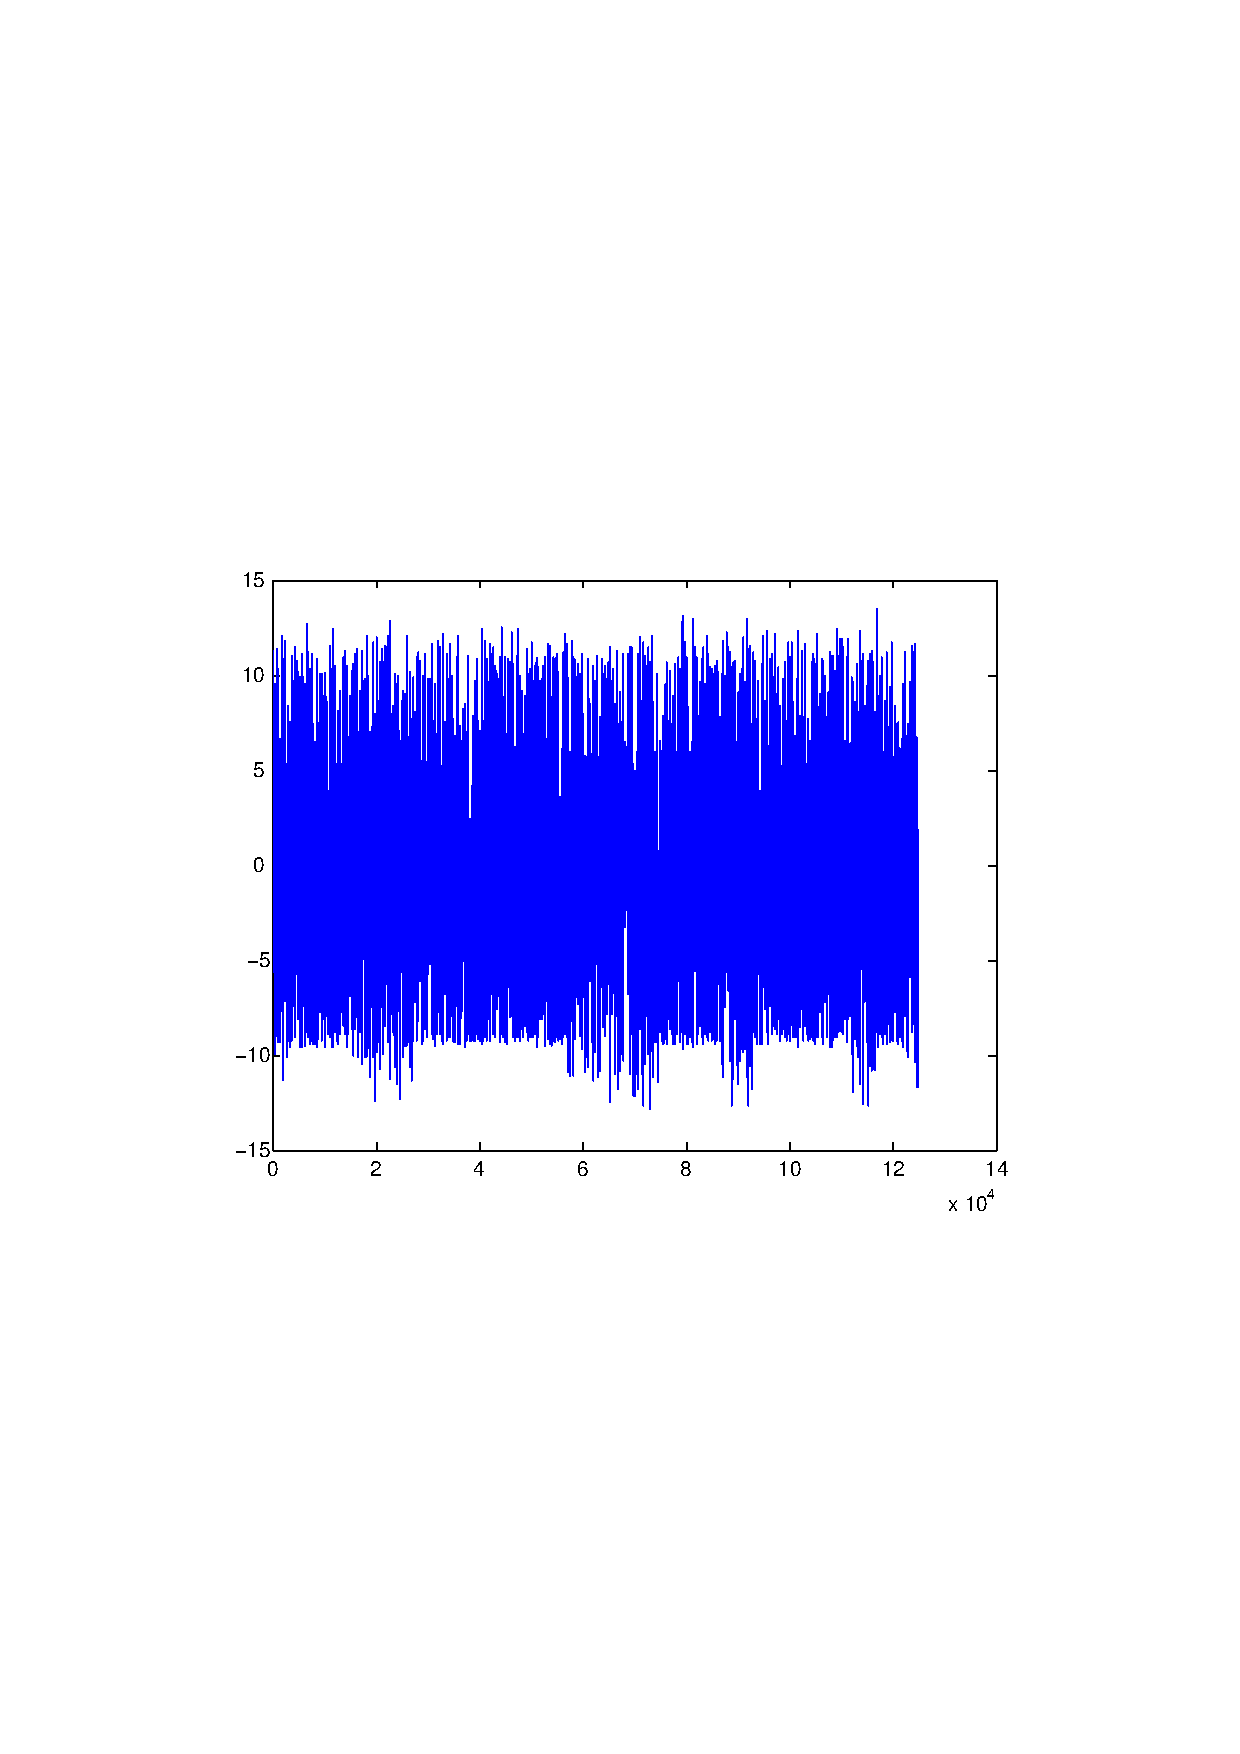
\includegraphics[scale=0.55, trim = 35mm 85mm 40mm 95mm, clip]{./Bilder/Rauschen0dB}
                           \caption{0dB Rauschen}
                       \end{figure}
        
                   \end{minipage}
        
                   \begin{minipage}{0.6\textwidth}
                       \begin{figure}[H] 
                           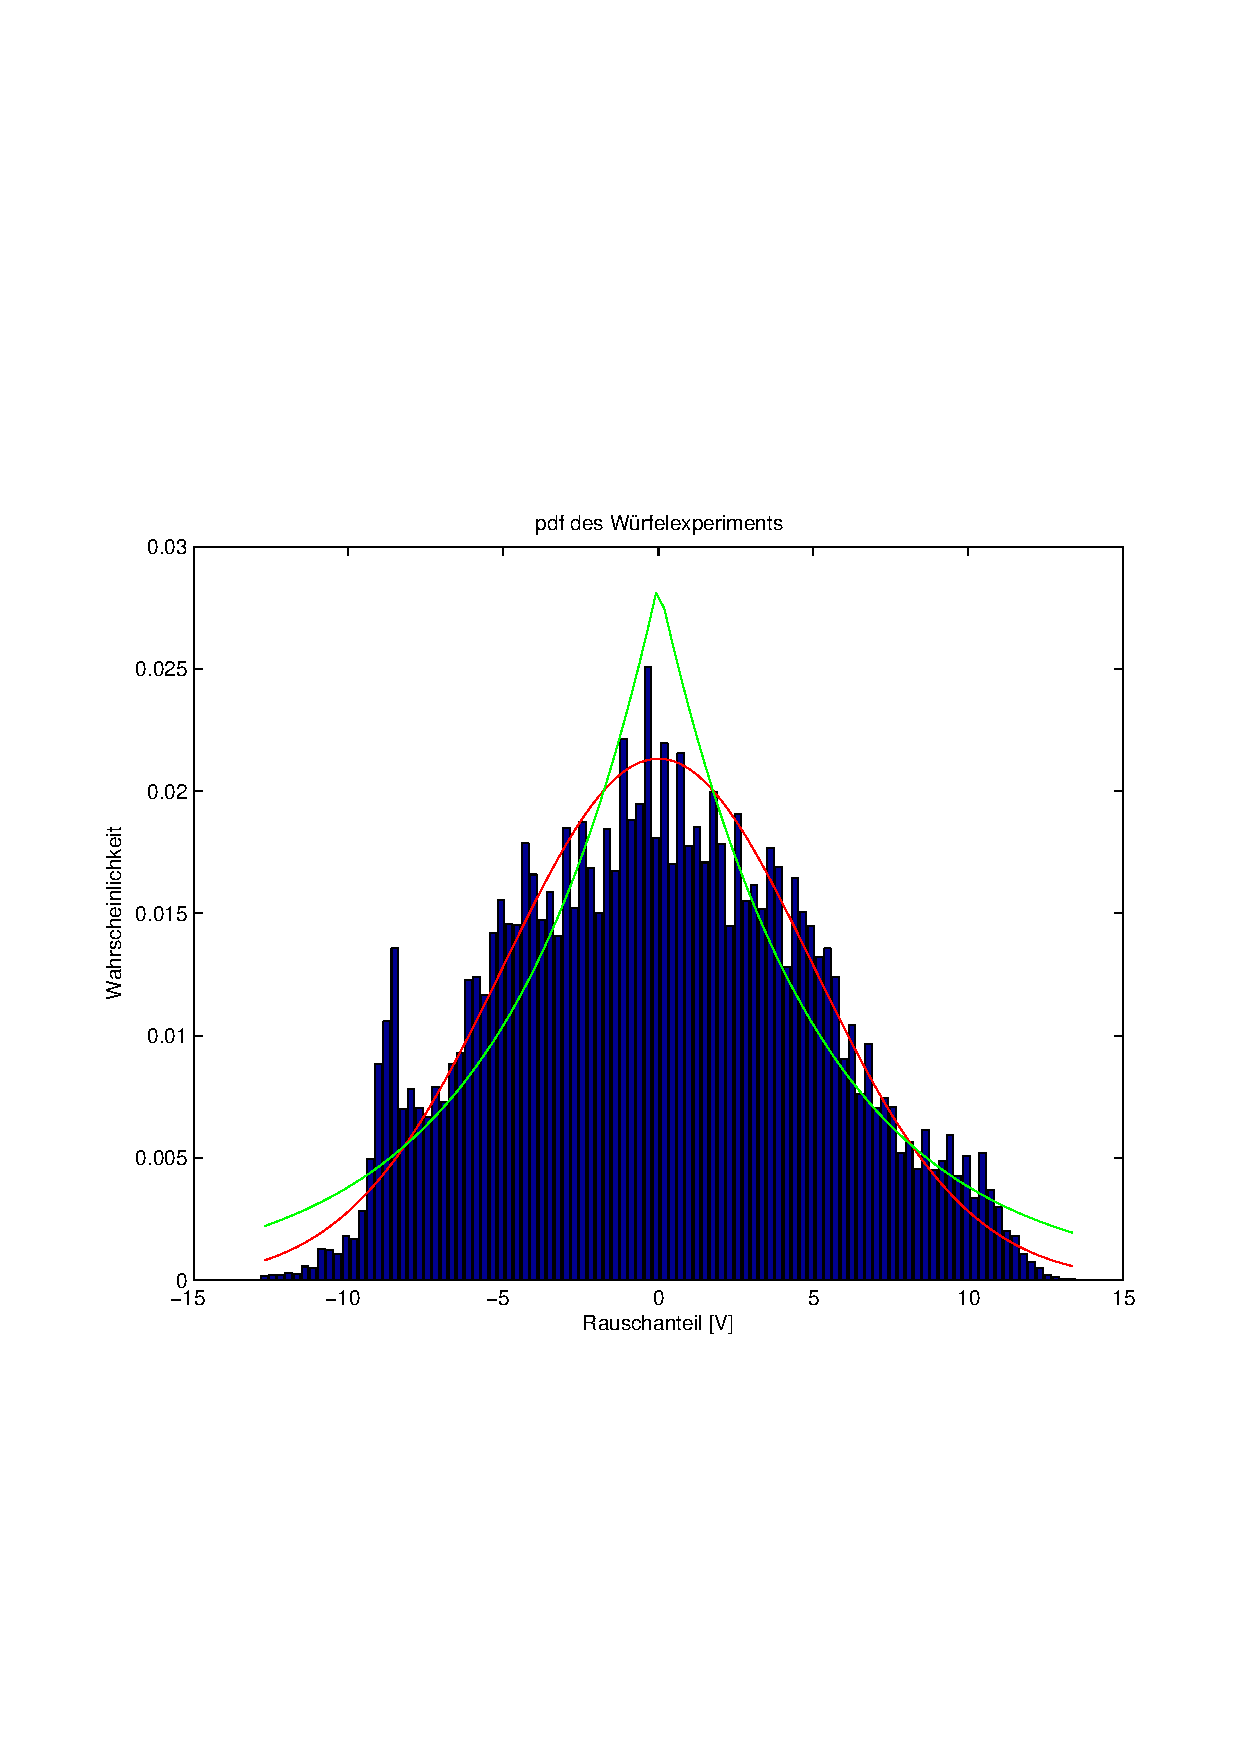
\includegraphics[scale=0.49, trim = 10mm 65mm 10mm 85mm, clip]{./Bilder/PDFRauschen0dB}
                           \caption{Häufigkeitsverteilung 0dB Rauschen}
                       \end{figure}
        
                   \end{minipage}
        
               \end{tabular}
               \end{center}

        
        Neben der Verteilungsdichtefunktion des Rauschanteils haben wir auch noch die dazugehörige Gaußverteilung (in
        Rot) sowie die dazugehörige Laplaceverteilung geplottet. Die Verteilung von dem $-20dB$ Rauschen lässt sich
        schwer einer der beiden Verteilungen zu zuorden. Die anderen beiden Verteilungen von dem $-6db$ sowie dem $0dB$
        Rauschen lassen sich der Gaußverteilung zuordnen. Daher liegt die Vermutung nahe, dass es sich bei der
        Verteilung bei $-20dB$ ebenfalls um eine Gaußverteilung handelt. \vspace{1em}
        
        
        Hier die Ergebniss der SNR-Messung:
            \begin{center}
                  \begin{tabular}{|c|c|}
                  \hline
                   Rauschen [dB] &  SNR [dB] \\ \hline 
                   $-20$ &  17.1228 \\ \hline
                   $-6$ &  2.9721 \\ \hline
                   $0$ &  -1.9448 \\ \hline           
                 \end{tabular}\vspace{1em}
                 
            \caption{SNR des Rauschens}            
            \end{center}
    
        Die Ergebnisse der Häufigkeitsverteilung entsprechen unseren Erwartungen. 
    
        Bei dem Signal-Rausch-Verhältniss fällt auf, dass bei $14dB$ mehr Rauschen das SNR um $14dB$ absinkt. Und
        genauso beim nächsten Schritt von $6dB$ fällt das SNR um $5dB$. Daher kann man schon von einem linearen
        zusammenhang sprechen. Ein solches Verhalten haben wir erwartet. 
        
    \end{quote}
\end{quote}
%--------------------------------------------------------------------
%--------------------------------------------------------------------

\end{document}
